\documentclass[11pt]{article}

\usepackage[a4paper,margin=2.35cm]{geometry}
\usepackage{booktabs}
\usepackage{graphicx}
\usepackage{hyperref}
\usepackage{url}
\usepackage{array}
\usepackage{caption}
\usepackage{microtype}
\usepackage{xcolor}
\usepackage{longtable}
\IfFileExists{placeins.sty}{\usepackage{placeins}}{\newcommand{\FloatBarrier}{\clearpage}}
\newcommand{\PDAOfficialOverlap}{227}
\newcommand{\PDAWeekTwoAccuracy}{0.9830}
\newcommand{\PDAWeekTwoMacroFOne}{0.9743}
\newcommand{\PDAMobileParams}{2.27M}
\newcommand{\PDAMobileFlops}{0.31G}
\newcommand{\PDAMobileThroughput}{644.3}
\newcommand{\PDAFinalAccuracy}{0.9953}
\newcommand{\PDAFinalMacroFOne}{0.9941}
\newcommand{\PDAErrorCount}{50}
\newcommand{\PDATestCount}{10709}
\newcommand{\PDAECE}{0.0965}
\newcommand{\PDAMCE}{0.3348}
\newcommand{\PDABrier}{0.0140}
\newcommand{\PDADemoLatency}{129.8}
\newcommand{\PDAVLMChoice}{11/15}
\newcommand{\PDAVLMCondition}{1/5}
\newcommand{\PDAWeekEightCleanTests}{226}


\definecolor{evidenceblue}{HTML}{0066CC}
\hypersetup{colorlinks=true,linkcolor=evidenceblue,urlcolor=evidenceblue,citecolor=evidenceblue}
\setlength{\emergencystretch}{2em}
\renewcommand{\arraystretch}{1.15}

\title{PlantDiseaseAI: From a High-Scoring Classifier to an Auditable Plant-Disease Research System}
\author{Panjoel}
\date{2026-07-19}

\begin{document}
\maketitle

\begin{abstract}
This paper reports the complete Week 1--8 research and engineering evidence for PlantDiseaseAI. The project combines a PlantVillage data audit, a unified five-model benchmark, controlled ablation, error and calibration analysis, Grad-CAM relevance visualization, an MPS/Streamlit demo, Apple container reproduction, and a small Qwen3-VL exploration. A later React/FastAPI serving path adds target-leaf selection, plant-identity routing, OpenCV morphology evidence, and abstention gates around the frozen classifier without changing its measured benchmark. In Week 2, ResNet50 reached Accuracy \PDAWeekTwoAccuracy{} and Macro F1 \PDAWeekTwoMacroFOne{} on the official split; MobileNetV2 provided an efficiency candidate with \PDAMobileParams{} parameters, \PDAMobileFlops{} FLOPs, and \PDAMobileThroughput{} img/s under the recorded MPS protocol. The Week 3 Label Smoothing plus Cosine Scheduler candidate reached Accuracy \PDAFinalAccuracy{} and Macro F1 \PDAFinalMacroFOne{} with seed 42 on the official split. However, the split audit identified \PDAOfficialOverlap{} overlapping leaf IDs, so the result is not evidence of entity-isolated generalization. Week 4 recorded \PDAErrorCount{}/\PDATestCount{} errors, ECE \PDAECE{}, MCE \PDAMCE{}, and Brier score \PDABrier{}. The Week 5 \PDADemoLatency{} ms value is one fixed synthetic CPU observation inside the container, not a general latency benchmark. In the Week 6 smoke study, Qwen3-VL choice/few-shot prompting reached \PDAVLMChoice{} exact match while the condition task reached only \PDAVLMCondition{}. The Week 8 clean lane passed \PDAWeekEightCleanTests{} tests and was complemented by local-evidence and Apple-container lanes. The central finding is not that a high score implies trustworthy diagnosis, but that model numbers become research evidence only when their data boundaries, negative results, reproduction conditions, and safety behavior are made explicit.
\end{abstract}

\section{Introduction}

Image classification can provide a low-cost entry point for plant-health screening, but high dataset accuracy does not automatically imply trustworthy field diagnosis. Trustworthiness requires at least four kinds of evidence: a stable data protocol, traceable metrics, explicit analysis of errors and confidence, and a serving interface that refuses claims outside the evaluated scope. PlantDiseaseAI therefore reframes the objective from ``train the highest-scoring model'' to ``build a research system that can explain when it works, when it fails, and how its evidence can be reproduced.''

The classification core was developed in stages. Week 1 fixed loading, label mapping, training, evaluation, and single-image inference. Week 2 compared five convolutional architectures under one protocol. Week 3 used single-factor ablation to support model selection. Week 4 audited errors, calibration, and Grad-CAM. Week 5 integrated Top-5 prediction, explanation, and safety messaging into a demo. Week 6 explored a vision-language model only after the classifier core was independently usable. Week 7 organized research communication, and Week 8 executed clean, local-evidence, and Apple-container reproduction lanes.

The contributions are fourfold. First, the work provides a comparable five-model benchmark and an ablation-based decision rather than a cherry-picked architecture. Second, it treats split overlap, per-sample errors, calibration, explanation-layer choice, and fixed-input latency as first-class evidence. Third, it links tests, model artifacts, figures, paper claims, and local container validation to one release candidate. Fourth, it separates verified classifier evidence from implemented serving gates and experimental extensions, allowing target-leaf, identity, morphology, and guidance stages to abstain without upgrading their evidence status. All conclusions remain bounded by the official split, one principal seed, and controlled backgrounds. The system is not presented as professional diagnosis and does not provide pesticide, dosage, or regulatory instructions.

\section{Related Work}

PlantVillage introduced an open repository of plant-health images\cite{hughes2015plantvillage}. Mohanty et al. demonstrated the potential of deep convolutional classification on these images while motivating caution about transfer to collection environments outside the dataset\cite{mohanty2016plantdisease}. PlantDiseaseAI uses the closed plant--condition labels but emphasizes split audit, negative-result retention, and explicit controlled-background limitations rather than attempting a new leaderboard claim.

The architecture benchmark covers ResNet\cite{he2016resnet}, MobileNetV2\cite{sandler2018mobilenetv2}, and EfficientNet\cite{tan2019efficientnet} families. Training factors include Label Smoothing\cite{szegedy2016label}, Focal Loss\cite{lin2017focal}, cosine scheduling\cite{loshchilov2017sgdr}, RandAugment\cite{cubuk2020randaugment}, Mixup\cite{zhang2018mixup}, and CutMix\cite{yun2019cutmix}. These methods are treated as hypotheses under a frozen budget; their negative and positive outcomes are preserved together.

Grad-CAM is used for class-related spatial visualization\cite{selvaraju2017gradcam}, but its heatmaps are not interpreted as causal explanations. Confidence analysis follows calibration work for modern neural networks\cite{guo2017calibration} and distinguishes top-label calibration from full multiclass calibration. The exploratory Week 6 branch uses the capabilities described by the Qwen3-VL-4B-Instruct model card\cite{qwen3vl2025modelcard}, with claims restricted to the observed local smoke workload.

\section{Dataset, Task, and Split Audit}

The verified task is 38-class whole-image classification. Each leaf image is mapped to one PlantVillage plant--condition class. A later serving layer produces heuristic target-leaf masks, lesion candidates, and morphology summaries, but these are not learned pathological segmentation, pathogen assays, or open-set guarantees. Random augmentation is restricted to training, while validation and test preprocessing is deterministic. The official test subset is excluded from checkpoint selection and hyperparameter search.

The project retains the data source's official train/test split and creates a stratified train/validation partition inside the training portion using seed 42. Identifier-level auditing found \PDAOfficialOverlap{} leaf IDs present across official train and test. The overlap is not necessarily pixel duplication, but it means correlated views of a leaf entity can cross the evaluation boundary. This paper therefore consistently says ``official-split result'' rather than ``leakage-free'' or ``entity-isolated'' result.

This finding changes the interpretation of every benchmark. A classifier may learn disease evidence, background regularities, and entity-correlated features. Controlled images do not cover field lighting, occlusion, viewpoint changes, camera shifts, unknown diseases, or non-leaf inputs. The highest-priority follow-up is therefore an entity-grouped frozen split followed by multi-seed and external-domain evaluation, not simply a larger architecture.

\subsection*{Audit decisions and a stronger split protocol}

The audit preserves the source label and split rather than silently rewriting either. A suspected overlap is recorded as a limitation because changing it after observing test performance would create a new protocol and invalidate direct comparisons with the completed runs. A stronger protocol should derive a stable entity key, group every correlated view under that key, and assign groups rather than images to train, validation, and test. The grouping rule, source revision, class counts, seed, and index files must be versioned before model selection.

Entity isolation alone is not enough. The new test set must remain untouched while architecture and training decisions use training and validation only. Class support needs review after grouping because rare classes can become too small for stable Macro F1. Duplicate checks should combine metadata and perceptual review, while uncertain cases remain in an audit ledger. Official-split and entity-isolated results should be reported side by side as different protocols, never merged into one headline value.

\section{Unified Training and Evaluation Protocol}

Training, evaluation, inference, and the demo share one label mapping, model factory, checkpoint interface, and deterministic test transform. The best checkpoint is selected by validation Macro F1 and evaluated on the official test split. Reported outputs include Accuracy, Macro Precision, Macro Recall, Macro F1, per-class scores, raw and normalized confusion matrices, and per-sample predictions. Macro F1 is a principal metric because each class receives equal weight.

The frozen Week 3 budget uses ResNet50, 224-pixel inputs, batch size 16, five epochs, AdamW, an initial learning rate of 0.001, and seed 42. A single-factor run changes exactly one factor; combined candidates are separately labeled. Randomness is seeded for Python, NumPy, PyTorch, and DataLoader workers. MPS efficiency measurements use float32, batch-1 latency, batch-32 throughput, 10 warmups, and 50 measured iterations. Peak memory is not claimed because the local MPS workflow does not provide the same reliable interface as CUDA.

Each formal run stores its resolved configuration, split and labels, environment, logs, metrics, and checkpoint index. The Week 8 manifest adds logical repository paths, sizes, and SHA-256 values for release evidence. Consequently, no metric in this paper should be detached from its seed, split, device, precision, and measurement protocol.

\subsection*{Protocol invariants and failure records}

The shared implementation prevents training, evaluation, inference, and Streamlit from maintaining separate preprocessing or label-order copies. Checkpoint loading validates model metadata and class count. Top-5 output is sorted and constrained to valid probabilities. Grad-CAM hooks have explicit lifecycles so repeated requests do not accumulate callbacks. These engineering invariants matter scientifically: a label-order mismatch or changed normalization can produce plausible but invalid outputs without changing model weights.

Runs are marked completed, failed, aborted, or smoke-tested. A failed run is not deleted, and a smoke check is not promoted to a full experiment. MPS reproducibility does not imply bitwise equality across devices, and a successful container health probe does not imply production load capacity. Encoding these distinctions prevents later public material from silently upgrading the evidence status.

\section{Five-Model Benchmark}

\begin{table}[htbp]
\centering
\caption{Week 2 model benchmark under a unified protocol}
\label{tab:week2-benchmark-en}
\resizebox{\textwidth}{!}{%
\begin{tabular}{lrrrrrr}
\toprule
Model & Test Acc & Macro F1 & Params & FLOPs & Latency & Throughput \\
\midrule
MobileNetV2 & 0.9760 & 0.9674 & 2.27M & 0.31G & 6.49 ms & 644.3 img/s \\
ResNet18 & 0.9774 & 0.9661 & 11.20M & 1.82G & 2.82 ms & 564.5 img/s \\
ResNet50 & 0.9830 & 0.9743 & 23.59M & 4.11G & 7.42 ms & 165.9 img/s \\
EfficientNet-B0 & 0.9804 & 0.9703 & 4.06M & 0.40G & 7.25 ms & 305.6 img/s \\
EfficientNetV2-S & 0.9794 & 0.9708 & 20.23M & 2.88G & 14.99 ms & 133.4 img/s \\
\bottomrule
\end{tabular}
}
\end{table}


ResNet50 led the unified benchmark with Accuracy \PDAWeekTwoAccuracy{} and Macro F1 \PDAWeekTwoMacroFOne{}, supporting its role as the high-accuracy ablation baseline. MobileNetV2, with \PDAMobileParams{} parameters, \PDAMobileFlops{} FLOPs, and \PDAMobileThroughput{} img/s in the recorded protocol, remained the efficiency candidate. The two architectures answer different questions: current accuracy under the project budget versus deployment-oriented resource trade-offs.

The latency and throughput values are comparable only within the recorded MacBook MPS setup, input size, precision, warmup, and repetition count. They cannot be directly transferred to mobile hardware, servers, or container CPU. Because all five architectures use the same split and evaluation protocol, they support internal selection, while the entity-overlap limitation applies to every row.

\subsection*{Accuracy--efficiency interpretation}

The benchmark has no universal winner. ResNet18 has lower batch-1 latency than MobileNetV2 in this MPS observation despite more parameters, showing that parameter count, FLOPs, latency, and throughput measure different bottlenecks. EfficientNet-B0 approaches ResNet50 accuracy with fewer FLOPs, while EfficientNetV2-S is not favored under the short budget. A deployment choice must specify its backend and workload instead of using parameter count as a proxy for every cost.

ResNet50 was selected because the next research question concerned controlled training changes, not because it was declared field ready. A fair efficiency study would export the same preprocessing and output contract, measure latency distributions and energy on the target device, and compare calibrated errors as well as speed. That study remains outside the current headline result.

\section{Controlled Ablation and Model Selection}

\begin{table}[htbp]
\centering
\caption{Completed Week 3 ablations and combined candidate, seed 42}
\label{tab:week3-ablation-en}
\resizebox{\textwidth}{!}{%
\begin{tabular}{llrrrr}
\toprule
ID & Method & Best epoch & Val Macro F1 & Test Acc & Test Macro F1 \\
\midrule
00 & ResNet50 baseline & 3 & 0.9775 & 0.9830 & 0.9743 \\
01 & Label Smoothing 0.1 & 5 & 0.9860 & 0.9885 & 0.9865 \\
02 & Focal Loss gamma 2.0 & 5 & 0.9776 & 0.9751 & 0.9652 \\
03 & Cosine Scheduler & 5 & 0.9959 & 0.9935 & 0.9898 \\
04 & EMA decay 0.999 & 5 & 0.9684 & 0.9752 & 0.9673 \\
05 & RandAugment & 5 & 0.9784 & 0.9765 & 0.9698 \\
06 & Random Erasing & 5 & 0.9718 & 0.9723 & 0.9683 \\
07 & Mixup alpha 0.2 & 5 & 0.9858 & 0.9837 & 0.9793 \\
08 & CutMix alpha 1.0 & 5 & 0.9868 & 0.9893 & 0.9863 \\
09 & Label Smoothing + Cosine & 5 & 0.9968 & 0.9953 & 0.9941 \\
\bottomrule
\end{tabular}
}
\end{table}


Cosine Scheduler was the strongest single factor, reaching Test Macro F1 0.9898. Label Smoothing and CutMix reached 0.9865 and 0.9863. Focal Loss, EMA decay 0.999, RandAugment, and Random Erasing underperformed the baseline under the five-epoch budget. These negative results suggest that hard-example weighting may amplify difficult or noisy cases, strong augmentation or erasing may remove fine lesion evidence, and slow EMA may lag during a short run.

Candidate 09 combines only Label Smoothing 0.1 and Cosine Scheduler. With seed 42 on the official split, which includes \PDAOfficialOverlap{} overlapping leaf IDs, it reached Accuracy \PDAFinalAccuracy{} and Macro F1 \PDAFinalMacroFOne{}. The decision is supported by two positive single-factor mechanisms affecting supervision and optimization, followed by an additional combined gain. Because multi-seed mean and dispersion are absent, this is a selected current candidate rather than evidence of a statistically stable improvement.

\subsection*{Why the controlled matrix matters}

The matrix separates targets, losses, schedules, weight averaging, image augmentation, and sample mixing. Without the single-factor runs, the final combination's gain could not be interpreted even provisionally: several methods effective elsewhere were harmful here. The schedule result is consistent with a short run benefiting from larger early steps and smaller late steps, while Label Smoothing reduces pressure toward extreme one-hot probabilities. This interpretation is a mechanism-level hypothesis, not causal proof.

The negative rows guide future work. Focal Loss should be revisited only after deciding whether low-F1 examples are genuine hard cases or overlap/annotation artifacts. RandAugment and Random Erasing need severity sweeps that preserve small lesion evidence. EMA needs a decay matched to update count. Mixup and CutMix change both input and soft target, so combining either with Label Smoothing requires a new matrix. Repeated tuning on the official test set would violate the protocol; these questions belong to entity-isolated validation.

\begin{figure}[tbp]
\centering
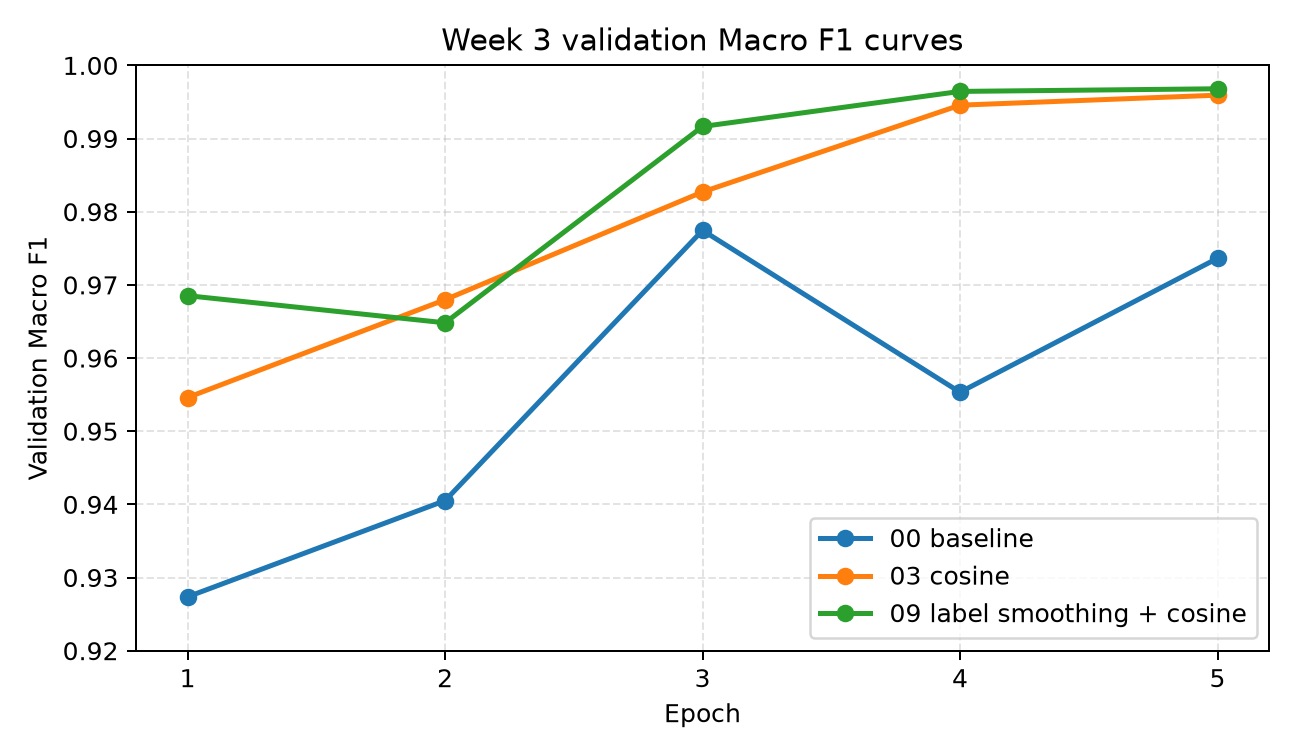
\includegraphics[width=0.88\textwidth]{../../reports/figures/week3_validation_macro_f1_curves.png}
\caption{Week 3 validation Macro F1 curves under the frozen budget. Optimization trajectories do not remove the single-seed limitation.}
\label{fig:week3-curves-en}
\end{figure}
\FloatBarrier

\section{Explainability, Error Analysis, and Calibration}

The selected candidate made \PDAErrorCount{} errors among \PDATestCount{} official test samples. Dominant confusions involved visually similar conditions, including corn gray leaf spot versus northern leaf blight and potato versus tomato late blight. Two errors remained above confidence 0.8. Per-sample auditing therefore reveals a failure mode that aggregate Accuracy alone hides: rare but confident mistakes.

\begin{table}[htbp]
\centering
\caption{Week 4 error and top-label calibration audit on the official split}
\label{tab:week4-analysis-en}
\begin{tabular}{p{0.44\textwidth}p{0.42\textwidth}}
\toprule
Audit item & Observation \\
\midrule
Test errors & 50 / 10709 \\
High-confidence errors (threshold 0.8) & Potato late blight $\rightarrow$ Tomato late blight (0.8475); Apple scab $\rightarrow$ Apple healthy (0.8322) \\
Top-label calibration & ECE 0.0965; MCE 0.3348; Brier 0.0140 \\
Interpretation boundary & Predicted-label confidence only; not full multiclass calibration or field reliability \\
\bottomrule
\end{tabular}
\end{table}


Top-label ECE was \PDAECE{}, MCE \PDAMCE{}, and Brier score \PDABrier{}. Most examples occupied high-confidence bins, where observed accuracy exceeded mean confidence, suggesting relative conservatism on this official split. The low-confidence bins were sparse, so the MCE peak should not be overinterpreted. No temperature scaling or full multiclass calibration was performed.

\begin{figure}[tbp]
\centering
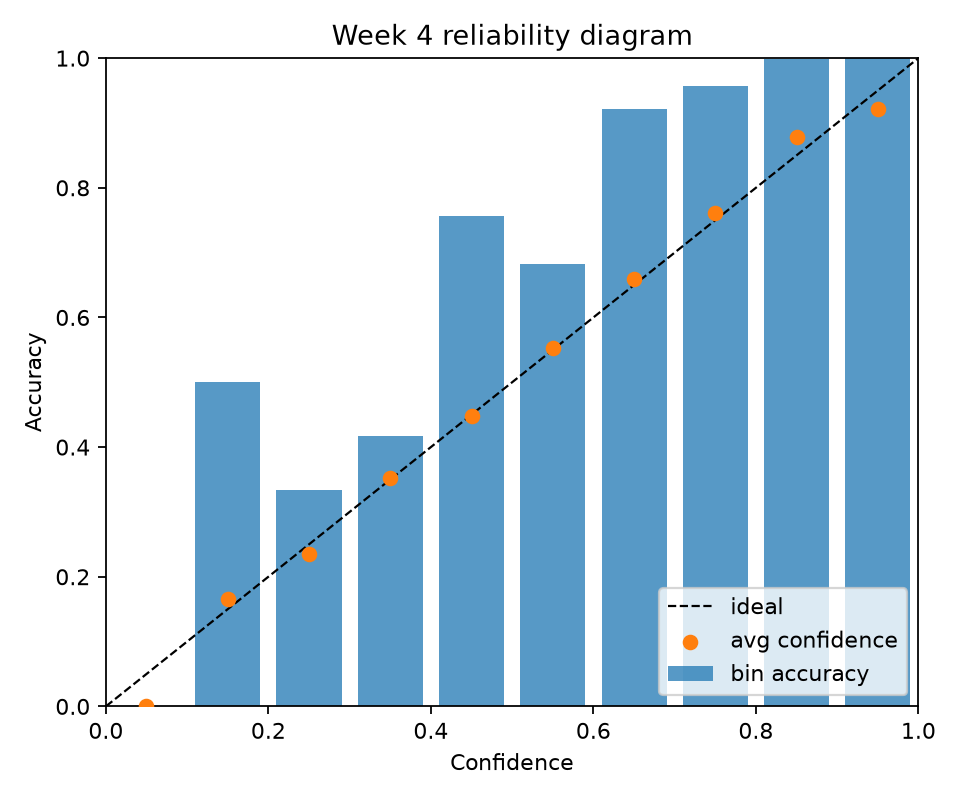
\includegraphics[width=0.63\textwidth]{../../reports/figures/week4_reliability_diagram.png}
\caption{Week 4 top-label reliability diagram. It compares predicted-label confidence and correctness, not field reliability.}
\label{fig:week4-reliability-en}
\end{figure}

The formal ResNet50 Grad-CAM target was corrected from the internal bottleneck tensor \texttt{layer4.2.conv3} to \texttt{layer4.2} after residual addition. The correction changed observed heatmaps but does not prove causal use of a lesion or the absence of background bias. A 24-example atlas covers correct/error and high/low-confidence groups. The review template exists, but complete human attention-region annotation is still pending.

\subsection*{Triangulating evidence}

The fixed atlas prevents selecting only attractive heatmaps. Correct/high-confidence cases test whether salient regions align with the leaf, error/high-confidence cases expose confidently wrong attention, and low-confidence groups show weaker evidence. Each sample records checkpoint, preprocessing, target class, target layer, and source index. A complete review should label lesion, healthy tissue, boundary, background, mixed, or uncertain attention and report reviewer agreement.

Calibration and Grad-CAM answer different questions. A calibrated probability does not show which pixels influenced it, while a leaf-centered heatmap does not guarantee a correct or calibrated result. Error counts reveal outcome failures but not their spatial mechanism. These artifacts are complementary observations. Future scoring should be preregistered before visual examples are interpreted numerically.

\begin{figure}[tbp]
\centering
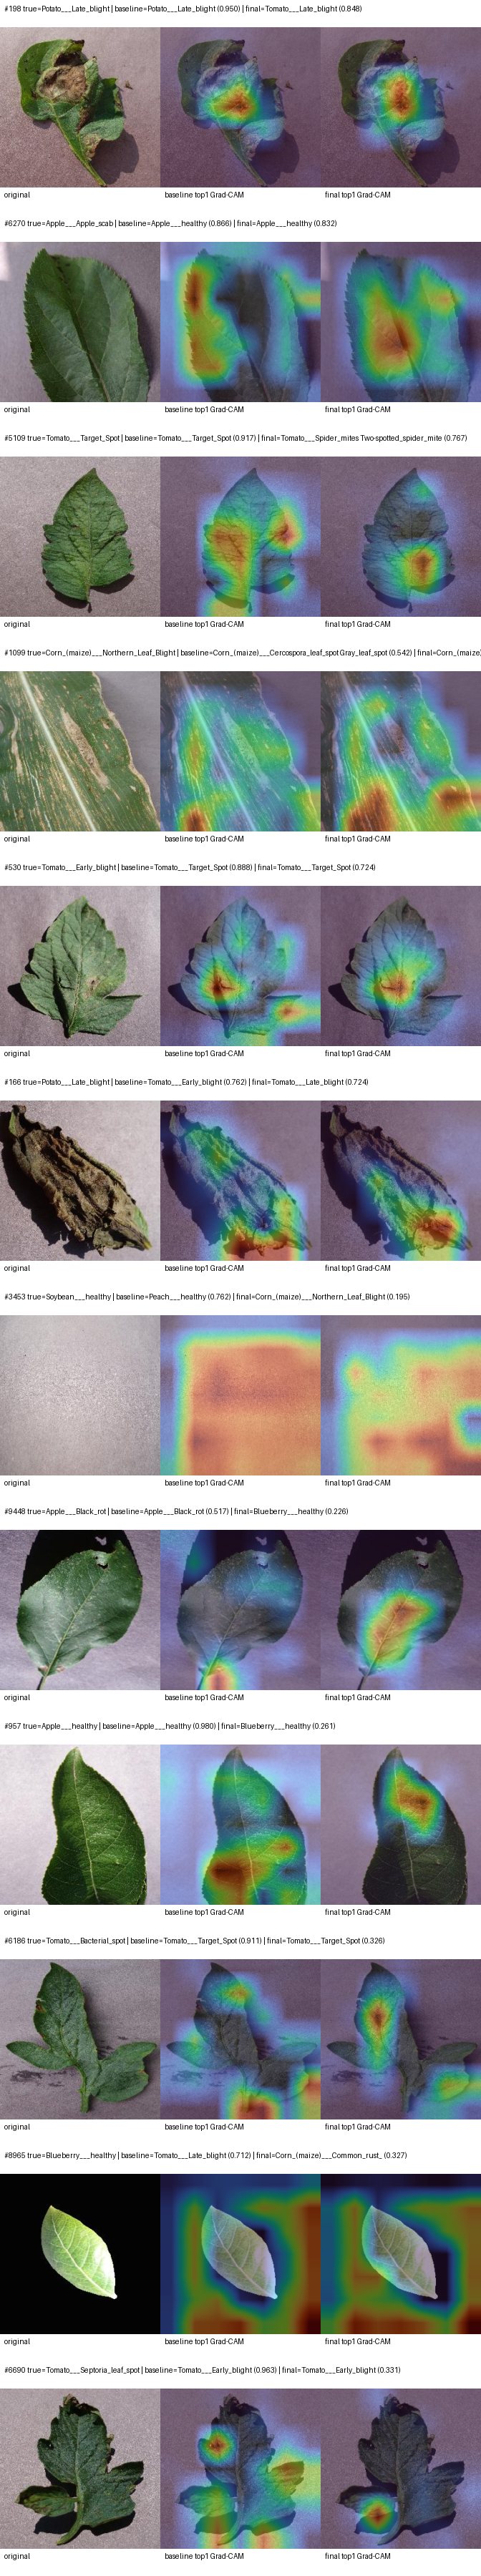
\includegraphics[height=0.62\textheight]{../../reports/figures/week4_baseline_vs_final_gradcam.png}
\caption{Frozen-example Grad-CAM comparison for the baseline and selected candidate. Heatmaps are relevance visualizations, not segmentation or causal evidence.}
\label{fig:week4-gradcam-en}
\end{figure}
\FloatBarrier

\section{Demo, MPS Serving, and Apple Container}

Week 5 packages byte-input validation, Top-5 ordering, probability and label mapping, low-confidence warnings, Grad-CAM overlays, and the non-professional-diagnosis notice into a UI-independent service used by Streamlit. Week 8 adds a React/Vite Liquid Glass interface while reusing the frozen checkpoint, labels, and preprocessing. The historical fixed synthetic input validates only the engineering path. The supplied field example has SHA-256 \nolinkurl{0364ff44229c70666216343057f9ae77d82438a7f842b30af1ffabb786061a7e}; it is an out-of-domain example with no verified ground truth.

\subsection*{Hierarchical serving and abstention}

The React/FastAPI path now selects one target leaf before model inference. It accepts a clearly dominant component automatically or a normalized source-image click, then applies click containment, foreground retention, coverage, border-contact, and elongated-axis purity checks. A failed or ambiguous mask returns an explicit selection request rather than forcing an image through the classifier. The accepted neutral-background cutout is shared by plant identity, condition inference, and Grad-CAM so hands, soil, sky, and neighboring plants are not directly visible to those models.

Identity routing first uses a local 114-class catalog built from UCI Leaf100 and the 14 PlantVillage hosts. This expands the routing vocabulary but is not validated 114-species open-world accuracy. Optional Pl@ntNet identity is called only when the local result is uncertain and a key is configured. A plant outside the supported PlantVillage hosts can retain an identity observation, but the disease path abstains. For a supported host, OpenCV records abnormal coverage, axis alignment, shape, coarse color, and spatial distribution as separate morphology evidence before crop-specific condition probabilities are exposed.

Accepted Corn inputs pass one additional central-axis gate. It checks abnormal coverage, central-axis share, longitudinal continuity, bilateral similarity, and off-axis discrete lesions before an infectious condition is selected. A positive pattern clears the infectious label, disease knowledge, diagnostic Grad-CAM, and management eligibility and reports only \texttt{suspected\_abiotic\_nutrient\_stress}. This is a conservative safety label, not confirmed nitrogen deficiency. Local Qwen is limited to visible morphology, and optional cloud management guidance remains locked whenever upstream identity, condition, or abiotic evidence does not support a disease claim.

\begin{figure}[tbp]
\centering
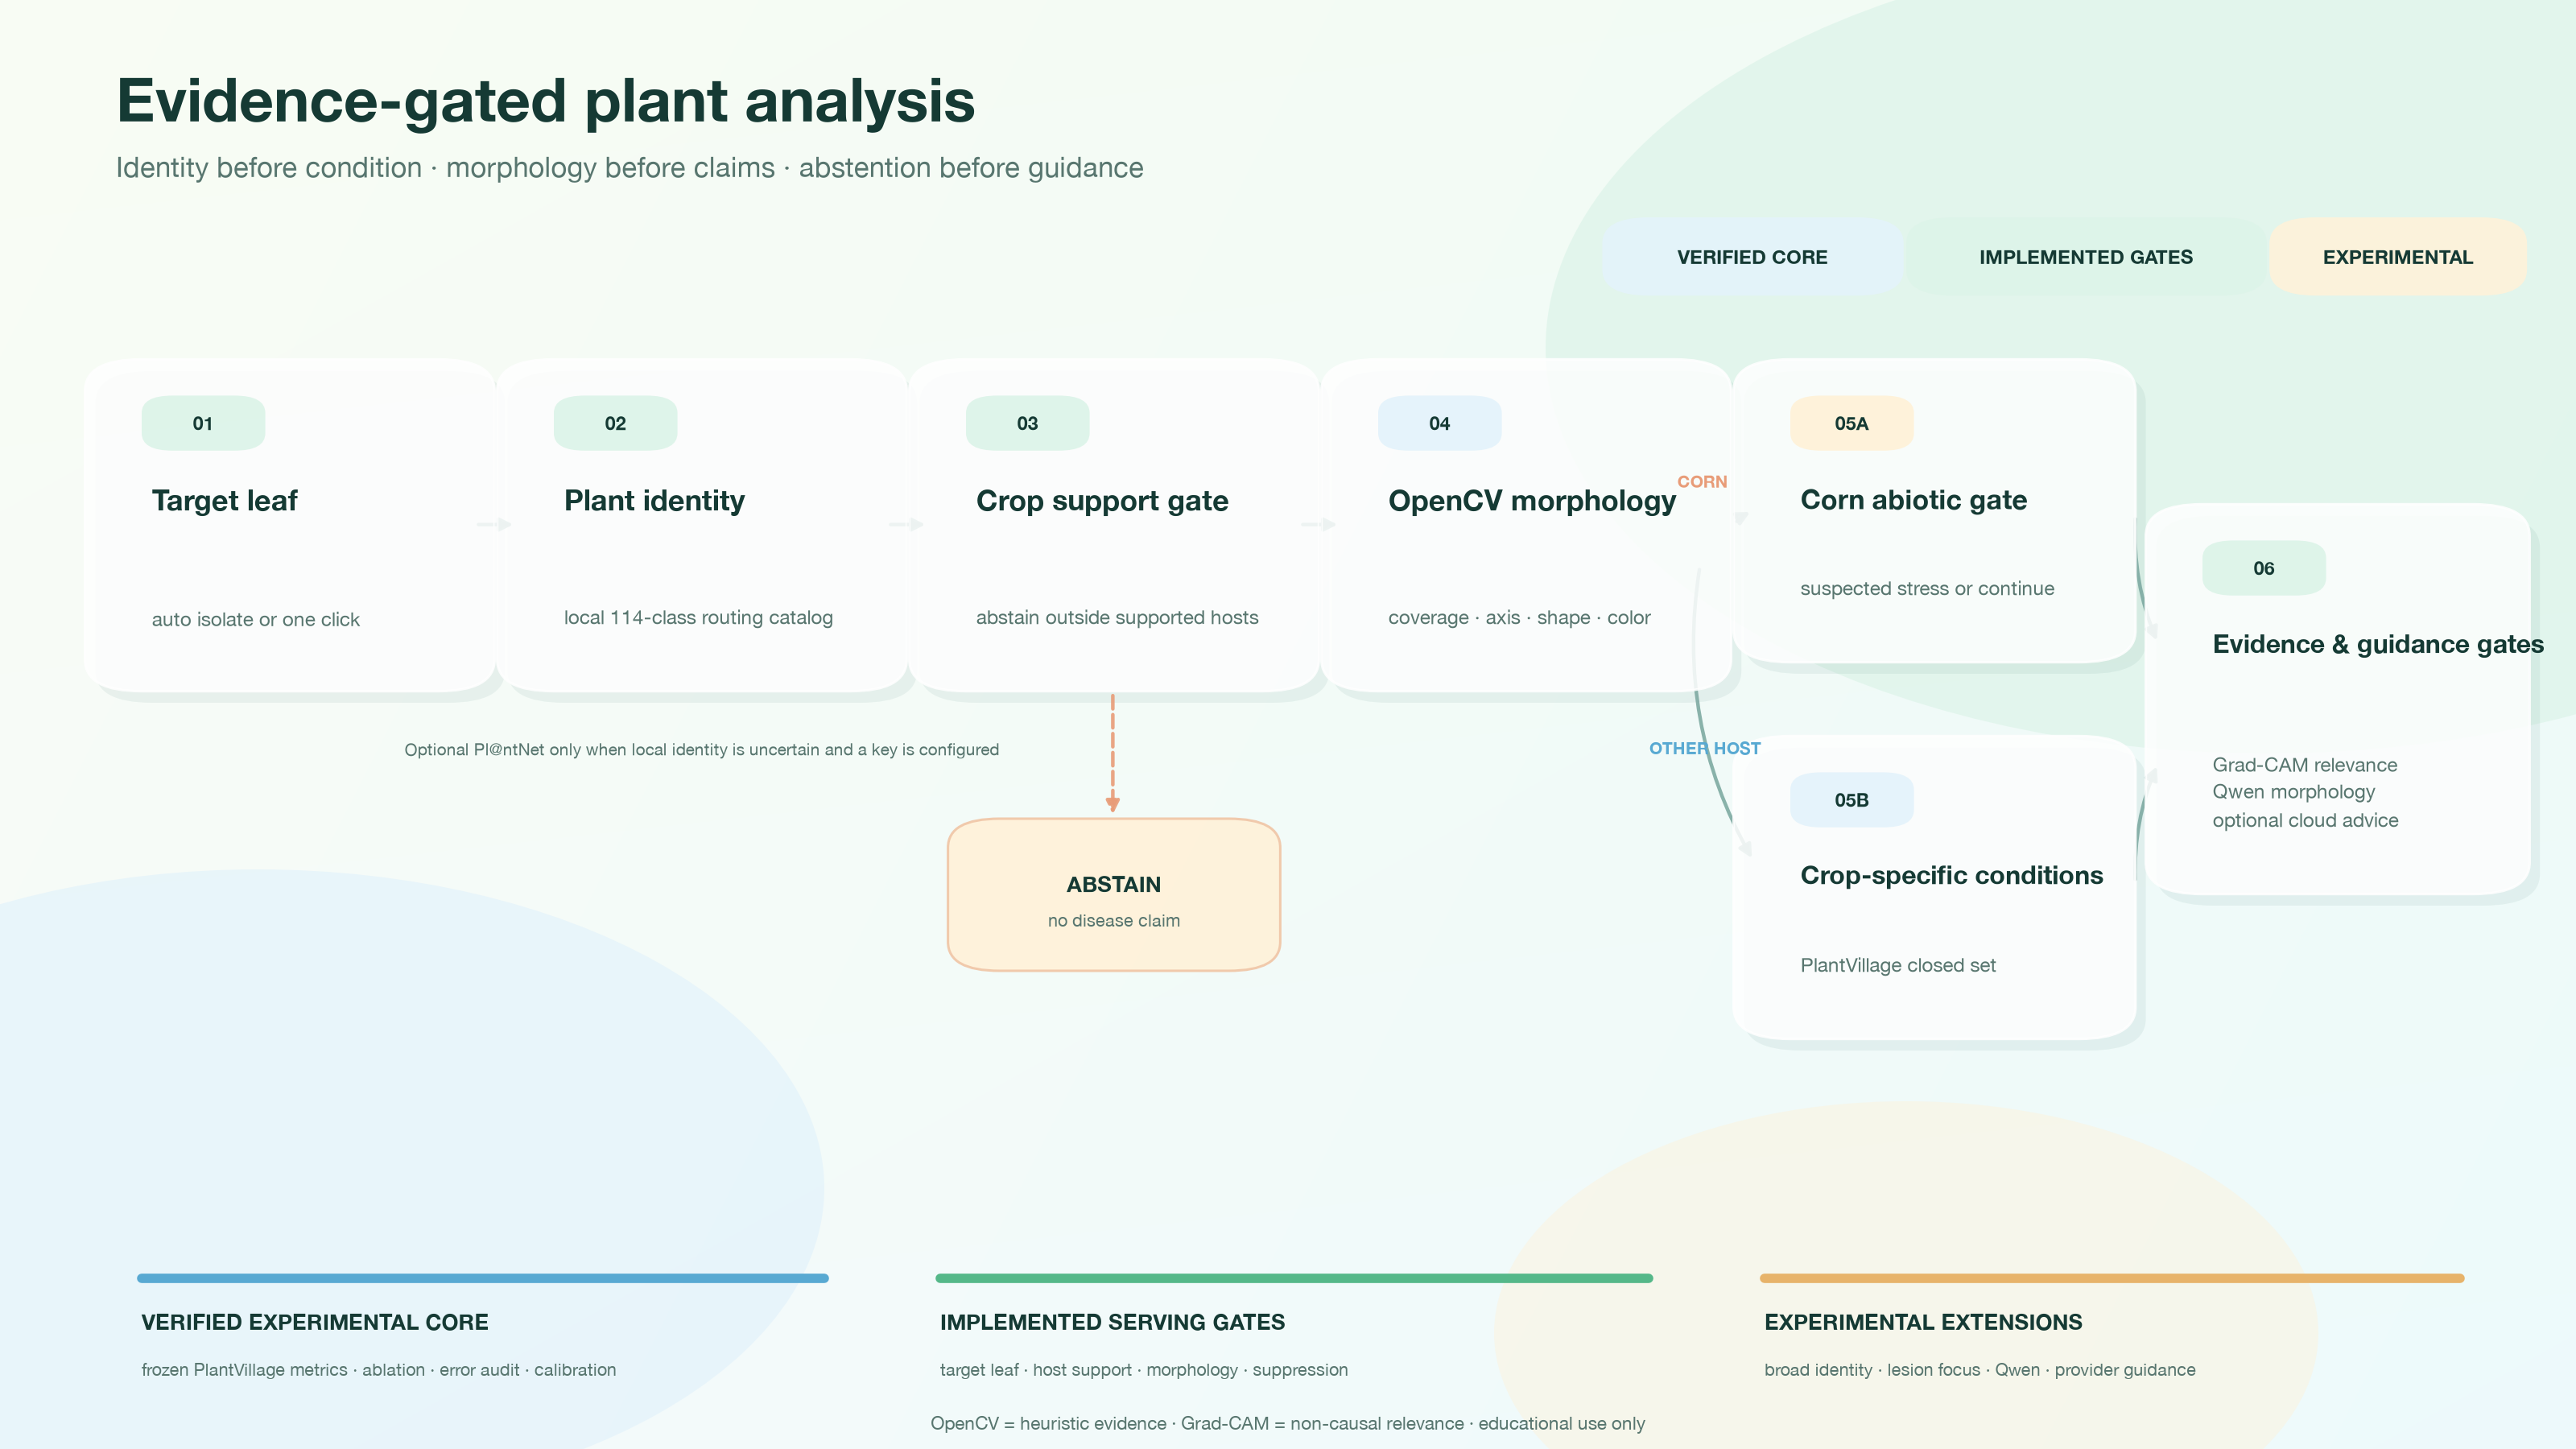
\includegraphics[width=0.98\textwidth]{../../docs/media/week8_hierarchical_serving_architecture.png}
\caption{Implemented hierarchical serving and safety gates around the frozen classifier. The diagram does not claim validated open-world identity accuracy, pathological segmentation, or confirmed nutrient diagnosis.}
\label{fig:hierarchical-serving-en}
\end{figure}

\begin{figure}[tbp]
\centering
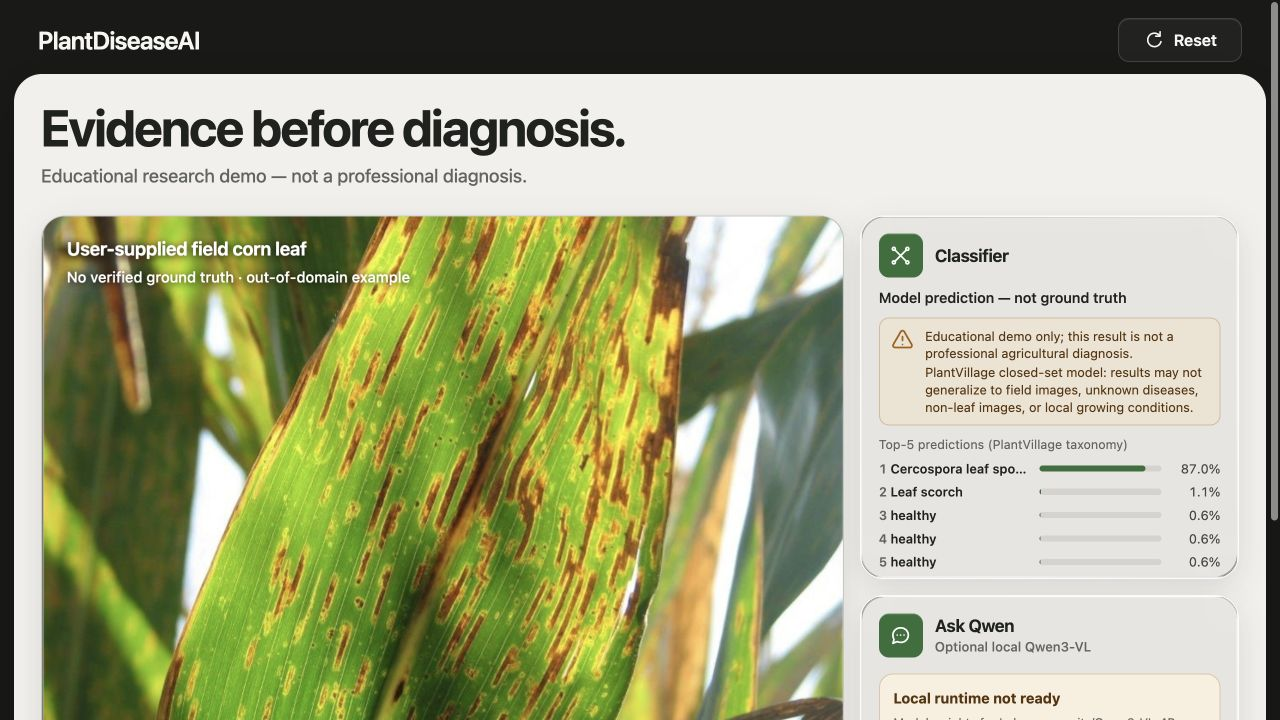
\includegraphics[width=0.94\textwidth]{../../reports/figures/week8_react_demo_desktop.png}
\caption{Browser-audited Week 8 React Demo. The ResNet-50/MPS value 0.870144 is a prediction, not truth or field-accuracy evidence; the image has no verified label and lies outside the controlled PlantVillage domain.}
\label{fig:week8-react-demo-en}
\end{figure}

MPS supports local inference and the Week 8 evidence recomputation. Apple container runs a linux/arm64 CPU image while the checkpoint is mounted from the host. The recorded \PDADemoLatency{} ms value is one total-time observation for the fixed synthetic input inside the Week 5 container, including prediction and Grad-CAM. It is not a repeated cold-start, cross-device, or production benchmark. A separate Week 8 MPS fixed-demo observation was 246.9 ms under different conditions and is not substituted for it.

\subsection*{Serving boundary and operational failures}

The service rejects empty, corrupt, and oversized byte inputs before inference. Low confidence adds a warning, but confidence cannot detect every out-of-distribution input. A non-leaf image can still receive a closed-set class because softmax distributes probability over known labels. The interface therefore states the PlantVillage domain independently of threshold and treats Top-5 alternatives as model outputs, not differential diagnoses.

Containerization reduces environment drift but adds a boundary: linux/arm64 CPU PyTorch cannot use the host MPS path as a native macOS process does. Model mount, port, architecture, image digest, and health endpoint are evidence. A production study would also require concurrency, memory, startup distributions, malformed-request load, and observability tests; none are inferred from this health probe.

\section{Qwen3-VL Exploration and Safety}

Week 6 explored Qwen3-VL-4B-Instruct through a local 4-bit MLX runtime after the classifier core was independently complete. Source images, not individual questions, define VQA split groups. The Week 8 optional panel targets \nolinkurl{mlx-community/Qwen3-VL-4B-Instruct-4bit}; default-cache weights were absent during browser QA, so \texttt{ready=false} and only the UI unavailable state were verified. Browser/API requests perform no automatic download. The assistant refuses ungrounded agricultural advice: low-confidence classifier context cannot become a definitive diagnosis, and pesticide, dosage, regulatory, or other high-risk actions are redirected to local plant-protection experts.

\begin{table}[htbp]
\centering
\caption{Week 6 Qwen3-VL smoke comparison (5 images and 15 questions)}
\label{tab:week6-vlm-en}
\begin{tabular}{lrrp{0.35\textwidth}}
\toprule
Prompt style & Exact match & Condition & Evidence boundary \\
\midrule
short free-form & 10/15 & 0/5 & Format improved, but unsupported pathogen terms appeared \\
choice & 11/15 & 1/5 & No automatic risk-word flags; fine-grained labels remained weak \\
few-shot choice & 11/15 & 1/5 & Tied with choice; this was not fine-tuning \\
\bottomrule
\end{tabular}
\end{table}


Choice and few-shot choice each reached \PDAVLMChoice{} exact match: plant and health status were 5/5, but fine-grained condition recognition was only \PDAVLMCondition{}. The short free-form prompt reached 10/15 and introduced unsupported virus, fungal, or bacterial terms. Structured options reduced free-form risk but did not solve disease recognition. The workload contained only five images and fifteen questions, with no LoRA/QLoRA training, complete human scoring, or field evaluation. It is therefore described only as a smoke exploration.

\subsection*{Requirements for a full VLM evaluation}

Strict exact match detects format errors in a closed task but is inadequate for open explanations. A full protocol should freeze entity-isolated images, define acceptable synonyms, and use blinded human rubrics for correctness, grounding, unsupported pathogen claims, refusal quality, and consistency with classifier confidence. Inter-rater agreement and failure examples should accompany automatic metrics. Advice questions require curated sources and jurisdiction-aware safety rules.

Few-shot prompting changes context only; it is not parameter training. LoRA or QLoRA would require a versioned training set, held-out entities, adapter configuration, resource logs, and fixed evaluation against zero-shot and classifier-assisted baselines. Since these artifacts do not exist, this paper excludes fine-tuning and capability-improvement claims.

\section{Week 8 Reproducibility Audit}

The Week 8 release candidate separates three complementary local lanes. Clean reproduction starts from locked dependency synchronization and runs static and full test checks. Local evidence uses the frozen checkpoint to regenerate metrics, Top-5 output, an MPS demo, and a Grad-CAM atlas. Apple container builds a linux/arm64 image and passes the Streamlit health probe. These lanes establish local, recorded reproducibility rather than public deployment availability.

\begin{table}[htbp]
\centering
\small
\caption{Week 8 local release-candidate reproduction lanes}
\label{tab:week8-repro-en}
\begin{tabular}{lp{0.19\textwidth}p{0.49\textwidth}}
\toprule
Lane & Status & Recorded evidence \\
\midrule
clean reproduction & passed & Locked environment sync, 226 tests, Ruff, and ty static checks \\
local evidence & passed & Frozen-checkpoint metrics, Top-5, MPS demo, and a 24-sample Grad-CAM atlas \\
Apple container & passed & linux/arm64 image build, Streamlit health probe, and local model mount \\
\bottomrule
\end{tabular}
\end{table}


The historical clean lane passed \PDAWeekEightCleanTests{} tests. The current delivery manifest records the refreshed source, environment, lock, checkpoint, and tracked artifacts. Clean, package, local-evidence, and container are \texttt{not\_run} for that source, so historical lane evidence is not inherited. It remains documented in \texttt{reports/week8\_reproducibility.md}. A claim ledger maps public numbers to evidence files and checks repository links. This candidate remains local; no remote release is created or published.

This design turns ``it runs'' into separate, testable events: environment synchronization, code checks, frozen-weight metric reproduction, explanation/demo generation, and container health. Status and limitation fields are preserved so an unexecuted task cannot silently become a passing claim.

\subsection*{Provenance and claim control}

Tracked evidence is separated from large local artifacts. The checkpoint remains outside ordinary source history but is identified by logical path, size, and SHA-256; the manifest does the same for reports and presentation inputs. A reviewer can detect a changed model or lock file without exposing a personal path. A missing required artifact fails the candidate rather than being replaced by an estimate.

The claim ledger maps locked values and approved wording to evidence and checks repository links. This is especially important for limitations: 0.9953 is acceptable only with seed-42 and official-split context, while 129.8 ms must retain its fixed synthetic CPU qualifier. Machine checks cannot judge every implication, so paper and slides still require human evidence review.

\section{Discussion and Negative Results}

The main technical finding is not that one architecture is universally best, but that different evidence supports different decisions. ResNet50 supports the high-accuracy research branch; MobileNetV2 supports resource trade-offs; cosine scheduling improved the short-budget optimization path; and Label Smoothing changed the supervision target. The declines from Focal Loss, EMA, RandAugment, and Random Erasing constrain the next search space and demonstrate that common techniques require protocol-specific evidence.

Errors, calibration, and Grad-CAM jointly show why Accuracy is insufficient. The 50 errors include confident failures, ECE/MCE depend on binning and a top-label definition, and target-layer choice materially changes heatmaps. Their combination yields better research questions but not causal conclusions.

The VLM study provides another useful negative result. Closed choices increased exact match to 11/15 and removed automatic risk-word flags, while condition recognition stayed at 1/5. More fluent language did not imply more reliable disease identification. The VLM is therefore an interaction branch with structured context and refusal behavior, not a replacement for the verified classifier core.

Together, the findings support a methodological lesson: reproducible agricultural AI is a loop, not a one-way sequence from model to demo. A data risk changes evaluation language; an error pattern suggests a new split; an explanation-layer correction changes the interpretation protocol; and a serving failure creates a new test. Week 8 closes the current loop locally while preserving the questions that should drive the next one.

\section{Limitations, Ethics, and Intended Use}

Eleven limitations remain binding. First, the official split contains \PDAOfficialOverlap{} overlapping leaf IDs and has no entity-isolated result. Second, the selected candidate is supported principally by seed 42, without multi-seed mean and variance. Third, controlled PlantVillage backgrounds do not represent field complexity. Fourth, Grad-CAM is relevance rather than causal, pathological, or segmentation evidence. Fifth, the 24-example attention review and 72-entry VQA template are not fully human-audited. Sixth, calibration is top-label only and has no post-hoc scaling. Seventh, container and local latency are condition-specific observations, not a production service-level objective. Eighth, OpenCV target and lesion regions are heuristic estimates rather than expert pathological masks. Ninth, the 114-class catalog has controlled-source pilot evidence but no validated 114-species field accuracy. Tenth, the Corn gate has no expert-labeled nutrient dataset and therefore cannot confirm nitrogen deficiency or another specific cause. Eleventh, the original user-supplied nitrogen-deficiency image is no longer present in the repository, so the recorded gate QA is not an external-image benchmark on that exact file.

Intended uses are research, teaching, and engineering demonstration: comparing training choices, showing closed-set Top-5 output, inspecting errors and explanation artifacts, and reproducing a local candidate. Excluded uses include independent field diagnosis, unknown-disease exclusion, pesticide selection or dosage, regulatory advice, commercial production decisions, or high-risk ecological actions. All user-facing material must retain the non-professional-diagnosis notice and refuse low-confidence, out-of-scope, or high-risk requests.

Data, models, and dependencies remain subject to their licenses. The paper cites public primary papers or the model card. Local weights, raw data, and personal paths are excluded from Git. Automated writing assistance cannot override experiment evidence; every final claim must trace to machine-readable results, logs, figures, or audit reports.

The planned next study should preregister its entity key and split before training, retain an untouched final test domain, and run several fixed seeds under equal budgets. It should report mean and dispersion for Accuracy and Macro F1, class-level uncertainty, and all failed runs. A field subset should cover lighting, clutter, viewpoint, crop stage, and acquisition-device metadata with consent and licensing recorded. These steps turn current limitations into testable research hypotheses rather than presentation disclaimers.

\section{Conclusion and Future Work}

PlantDiseaseAI now forms a local loop from data audit, unified benchmarking, ablation selection, per-sample errors, calibration, and Grad-CAM through an MPS demo, Apple container, VLM smoke exploration, Week 8 release audit, and a later evidence-gated React/FastAPI serving hierarchy. The selected candidate reports Accuracy \PDAFinalAccuracy{} and Macro F1 \PDAFinalMacroFOne{} with seed 42 on the official split; those values must always be presented together with the \PDAOfficialOverlap{}-entity overlap risk. The project's research value comes from evidence boundaries rather than expanding a high score, a heuristic mask, or a broad identity catalog into a field-reliability claim.

The next work is ordered as follows: create a leaf-entity-isolated frozen split; run multiple seeds and report dispersion; acquire legally sourced field-domain data; collect expert-labeled biotic, abiotic, and nutrient-stress regions; evaluate target-leaf and lesion masks against region annotations; complete Grad-CAM and VQA human review; evaluate refusal and open-set inputs; and consider LoRA/QLoRA only under a fixed test protocol and adequate resources. New results should enter a versioned manifest and claim ledger before entering papers, slides, or resumes.

\section*{Tool Disclosure}

Codex was used for code and document assistance, structural checking, and build automation. Panjoel is the sole author and remains responsible for experiment design, evidence selection, interpretation, final wording, and all research claims. Codex is not a co-author.

\bibliographystyle{plain}
\bibliography{../references}

\end{document}
